\documentclass[a4paper,12pt]{article}
\usepackage{graphicx}
\usepackage[UTF8]{ctex}
\usepackage{fontspec}
\usepackage{booktabs}
\usepackage{float}%浮动体
\usepackage{amsmath,amssymb}
\usepackage{fancyhdr}
%\usepackage{xcolor}
\usepackage{colortbl}
\usepackage{geometry}
\geometry{top=2cm,bottom=2cm,left=1cm,right=1cm}
\begin{document}
	\begin{figure}[H]
	\begin{center}
		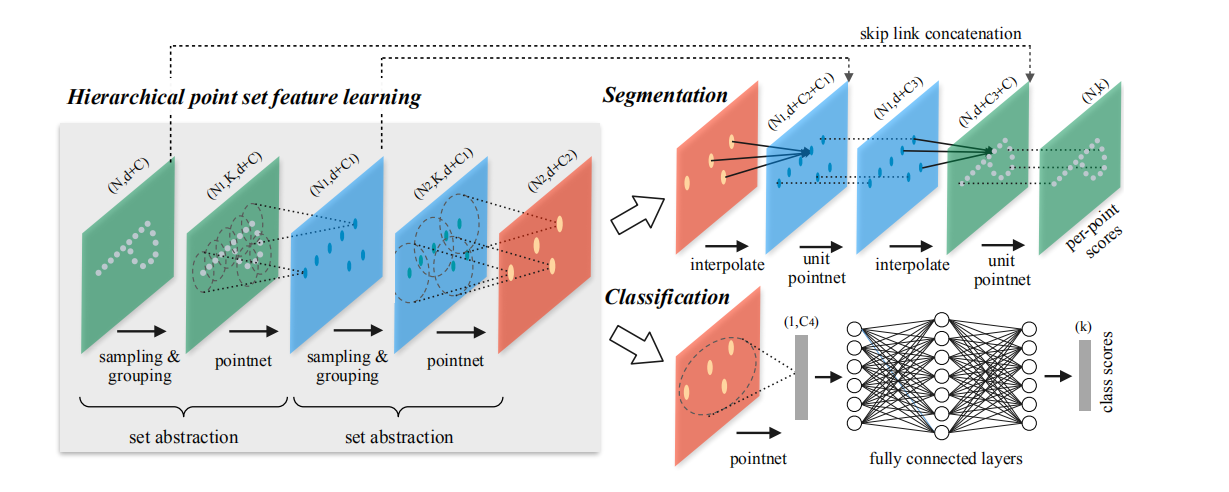
\includegraphics[width=0.9\textwidth]{img/PointNet++.png} 
		\caption{PointNet++}
	\end{center}
\end{figure}


\begin{itemize}
	\item 集合收缩:由抽样,组合,小型集合进行用$PointNet$特征提取
	\item  集合扩张:由插值和单元pointnet(few share fc and relu)
\end{itemize}
\textbf{抽样}:使用FPS(最远点抽样):\\
1、N个点中随机选取一个点a1,计算其余点到它的距离,选取距离最远的那个点(a2)加入集合{a1,a2}\\
2、随后计算其余N-2个点到该集合的距离(选取到该集合某个点最短距离),又选择其中一个最远的加入集合{a1,a2,a3}\\
3、如此往复,直到抽样K个点为止
\\
\textbf{多尺度组合}:因为点云各个地方的密集程度不同,导致密集程度不同的地方学习的特征有出入。\\
\textbf{组合}:球形查询(给定一个半径)或者KNN
\\
\textbf{插值}:
$$f^{(j)}(x)=\frac{\sum_{i=1}^{k} w_{i}(x) f_{i}^{(j)}}{\sum_{i=1}^{k} w_{i}(x)} \quad$$ where $\quad w_{i}(x)=\frac{1}{d\left(x, x_{i}\right)^{p}}, j=1, \ldots, C$.然后将收缩阶段的特征叠加在插值之后的特征中。
\paragraph{分类任务}
通过集合收缩之后,对余下的所有点进行一次PointNet提取特征,然后用FC 对其进行分类
\paragraph{语义分割} 在分类任务提取整体特征的基础上,通过插值和skip link connection还原成原始的points个数。


\end{document}